\section{Higher-dimensional history complexes}\label{sec:complexes}
\subsection{Commuting swaps and route cubes}
\begin{lemma}[Independence Lemma]\label{lem:indep}
Let $h$ be a history and $i_1<\dots<i_d$ positions with $i_{k+1}\ge i_k+2$ such that the pair $(N_{i_k},N_{i_k+1})$ consists of distinct labels whose exchange is legal in $h$. Then for every $b\in\{0,1\}^d$ the history $h_b$ obtained by performing the chosen exchanges is admissible and has the same endpoint, and the $h_b$ are pairwise distinct. They are the vertices of a $d$-cube whose edges are single legal swaps.
\end{lemma}
\begin{proof}
Induct on the blocks left to right. Both orders of the $k$-th pair lead to the same state, so the state before the $(k+1)$-st pair does not depend on the choices already made; legality of the $(k+1)$-st exchange is a statement about that state only (\cref{prop:diamond}(c)) and holds in every variant. All other letters are unchanged. The words are pairwise distinct since they differ in at least one of the chosen pairs.
\end{proof}
\prov{CW-0340}{D-T3}{PROVED}{FULL}
\begin{theorem}[route cubes of $72^r$]\label{thm:cube}
For every $r\ge1$ the complete histories ending at $72^r$ contain an $r$-cube: from the source $1$, the prefix $1^r$ followed by $r$ blocks, each independently $(1,2)$ or $(2,1)$.
\end{theorem}
\begin{proof}
After the prefix the state is $4^r$; block $j$ starts at $4^r\,18^{j-1}$, which is even, so $AB=2$ divides it and the exchange $(1,2)\leftrightarrow(2,1)$ is legal by \cref{prop:diamond}(c). Each block multiplies by $R(1)R(2)=18$, so all $2^r$ histories end at $4^r18^r=72^r$, and \cref{lem:indep} applies.
\end{proof}
\begin{proposition}[the cube dimension of $72^r$ is not $r$; finite-exact]\label{prop:cubedim}
Let $\delta(r)$ be the maximum cube dimension (the largest number of pairwise non-overlapping legal swaps in one history) over the complete histories of $72^r$. Then $\delta(1),\dots,\delta(4)=1,2,4,5$; trivially $\delta(r)\le\lfloor l/2\rfloor$ for a history of length $l$. An explicit $4$-cube in $72^3$: source $3$, word $(3,1,2,1,2,1,2,1)$, legal exchanges at the position pairs $(1,2),(3,4),(5,6),(7,8)$, endpoint $3\cdot\frac{16}3\cdot4^4\cdot(\frac92)^3=72^3$. \stat{finite-exact} for $r\le4$.
\end{proposition}
\begin{remark}[local does not imply global at overlaps]\label{rem:hexagon}
\Cref{lem:indep} concerns non-overlapping exchanges. For overlapping exchanges the braid hexagon of three distinct labels $N_1,N_2,N_3$ needs all six arrangements, which by \cref{prop:sat} happens iff $N_1N_2N_3\mid m$. The history $(2;1,2,4)$ ($2\to8\to36\to225$) has both adjacent exchanges legal ($(2,1,4)$ and $(1,4,2)$ are admissible) but only $3$ of the $6$ arrangements are admissible, since $8\nmid2$; and for $m=60$ the labels $2,6,10$ are pairwise exchangeable ($12,20,60\mid60$) while $120\nmid60$.
\end{remark}

\subsection{The histories of \texorpdfstring{$72^r$}{72 to the power r}: classes, groups and homology}
\begin{table}[tbp]\centering\small
\begin{tabular}{@{}lrrrrl@{}}\toprule
$r$ & histories & swap classes & $(m_0,\text{content})$ groups & max cube dim.\ & $\beta_*(Q)$ ($\mathbb F_2$)\\\midrule
1 & 4 & 3 & 3 & 1 & $(3)$\\
2 & 100 & 22 & 22 & 2 & $(22,7)$\\
3 & 3\,601 & 142 & 141 & 4 & $(142,368,3)$\\
4 & 194\,864 & 1\,114 & --- & 5 & ---\\\bottomrule
\end{tabular}
\caption{\textbf{Swap-class structure of the complete histories of $72^r$ (finite-exact).} Classes are counted over all (squarefree) sources. $Q$ is the cubical route complex whose vertices are all complete histories of $72^r$ and whose cells are sets of independent legal swaps; its $f$-vectors are $(4,1)$, $(100,96,11)$ and $(3601,6366,2832,294,4)$ (Euler characteristics $3$, $15$, $-223$ agree with the Betti vectors). The class counts for $r\le3$ and the cube dimensions for $r\le 4$ agree with the programme's records; the value $1\,114$ for $r=4$ and the complex $Q$ were computed in this work.}\label{tab:72r}
\end{table}
\begin{figure}[tbp]\centering
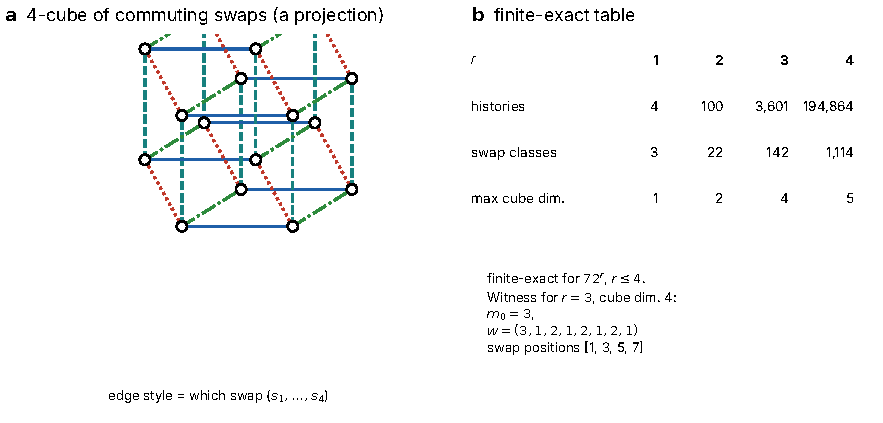
\includegraphics[width=\textwidth]{fig14_commuting_swaps}
\caption{\textbf{Commuting swaps and cubical faces (finite-exact data; the cube is drawn in projection).} (a) A projection of the $4$-cube formed by the sixteen histories obtained from the witness of \cref{prop:cubedim} by performing any subset of its four commuting exchanges; the four edge styles are the four exchanges $s_1,\dots,s_4$. It is a combinatorial $4$-cell and is not embedded in a Euclidean space of dimension $4$ by the drawing. (b) The table of \cref{tab:72r}.}\label{fig:cubes}
\end{figure}
\noindent The figure above is \cref{fig:cubes}; its caption states the exactness of what is drawn.
For $r=3$ the source-and-content groups number $141$ and the swap classes $142$: exactly one group of histories (source $15$, content $\{2,4,5,5,15\}$, endpoint $72^3$, two classes of four histories each) splits into two classes; for $r\le2$ classes and groups coincide. Over all non-squarefree endpoints $t\in[4,6000]$ with $H(t)\le4000$ (2\,354 endpoints), the endpoints at which some group of histories splits are exactly $1944,2400,4050,4320,5400$ (the first two sources of the pattern: source $2$, content $\{1,2,3,8\}$, endpoint $1944$, two classes of sizes $4$ and $1$; and the family of \cref{ex:src14}, endpoint $5400$). \stat{finite-exact}.
\prov{CW-0343}{D-T6}{FINITE-EXACT}{FINITE}
\begin{remark}[cube dimension is not homological degree]\label{rem:cubedeg}
The cube of \cref{thm:cube} is contractible, and a $d$-cube of commuting swaps contributes no homology of degree $d$ by its presence. For $r=3$ the complex $Q$ has cubes of dimension up to $4$ (four of them) but $\mathbb F_2$-Betti numbers $(142,368,3,0,0)$: homology lives in degrees $0,1,2$ only. The combinatorial cube dimension is an upper bound on the dimension of a cell, not an indication of any homological degree.
\end{remark}
\begin{proposition}[finite-exact: the groups are not always the classes]\label{prop:splitgroup}
The histories $(15;5,4,5,2,15)$ and $(15;15,2,4,5,5)$ have the same source, content $\{2,4,5,5,15\}$ and endpoint $72^3$ and lie in different swap classes; likewise $(2;1,2,3,8)$ and $(2;1,8,3,2)$ (endpoint $1944$).
\end{proposition}

\subsection{Dimension of an obstruction}
Let $C$ be a set of distinct labels and $m$ a source. Three numbers are attached to $(C,m)$: $d_{\mathrm{span}}=\rank_{\mathbb Q}\{\Delta(N):N\in C\}$ (the rank of the displacement vectors over \emph{all} primes); $d_{\mathrm{con}}=$ the number of primes $p$ such that relaxing the constraint at $p$ (replacing $v_p(m)$ by $\infty$, i.e.\ dropping $p$ from the thresholds) changes $\mathcal A(m)$; and $d_{\mathrm{top}}=$ the least size of a set $S$ of primes such that keeping only the constraints at $S$ preserves the Betti vector of $K_m$.
\begin{theorem}[passive coordinates]\label{thm:passive}
A prime that divides no label of $C$ never constrains: $\Delta_p(N)=2v_p(N+1)\ge0$ for $N\in C$, so $b_p(w)=0$ for every word $w$ over $C$. Hence admissibility, and every complex built from it, depends only on the active primes $\{p:p\mid N\text{ for some }N\in C\}$.
\end{theorem}
\begin{proof}
Immediate from \cref{thm:threshold}: $S_j(p)\ge0$ for all $j$.
\end{proof}
\prov{CW-0383}{B-T1}{PROVED}{FULL}
\begin{proposition}[the three dimensions differ]\label{prop:dims}
For $\{2,3,8,9\}$ at $72$: $(d_{\mathrm{span}},d_{\mathrm{con}},d_{\mathrm{top}})=(3,2,2)$; for $\{2,3,8,9,14\}$ at $1008$: $(4,2,2)$. In the first case the displacement vectors live in the primes $2,3,5$ (since $9+1=10$) and the active primes are $2,3$; in the second the displacement span has rank $4$ in the primes $2,3,5,7$, the active primes are $2,3,7$, the prime $7$ never constrains at $1008$ ($v_7(1008)=1$ and only the label $14$ consumes it), and the obstruction (the void of \cref{ex:void}) is already carried by the constraints at $\{2,3\}$.
\end{proposition}
\begin{proof}
Explicit exact computation: the ranks of the $\Delta$-matrices are $3$ and $4$; relaxing $2$ or $3$ changes $\mathcal A(m)$ and relaxing $7$ does not; keeping only the constraints at $\{2,3\}$ reproduces the Betti vectors $(1,1,0)$ and $(1,0,1,0)$, and no single prime does. See \cref{app:examples}.
\end{proof}
\prov{CW-0384}{B-T2}{PROVED}{FULL}
A rank-$4$ valuation realisation therefore carries a void whose obstruction is $2$-dimensional in the sense of constraints: the rank of the valuation span is not an obstruction dimension.
\begin{proposition}[irreducible multi-prime obstructions]\label{prop:irred}
Each of the following four statements about the route complex $K_m$ is an exact finite fact (replayed in \texttt{checks/}, with the admissible sets listed in \cref{app:examples}). For the content $C$ and source $m$ below, $K_m$ has the stated feature; and relaxing the constraint at any \emph{single} active prime makes $K_m$ contractible (Betti vector $(1,0,\dots,0)$), so every active prime is essential and the obstruction is genuinely $3$- (resp.\ $4$-)dimensional.
\begin{center}\small
\begin{tabular}{@{}llll@{}}\toprule
feature & content $C$ & source $m$ & active primes (all essential)\\\midrule
2 components & $\{2,3,4,5,6\}$ & $4$ & $2,3,5$\\
2 components & $\{2,3,4,5,6,7\}$ & $4$ & $2,3,5,7$\\
loop $(\beta_1=1)$ & $\{2,3,4,5,8\}$ & $32$ & $2,3,5$\\
loop $(\beta_1=1)$ & $\{2,3,4,5,6,7\}$ & $24$ & $2,3,5,7$\\\bottomrule
\end{tabular}
\end{center}
\end{proposition}
\prov{CW-0385}{B-T3}{PROVED}{FULL}
\emph{Irreducible means: relaxing any one active prime removes the obstruction.} In these examples the obstruction is a conjunction of independent single-prime blockers (every single relaxation trivialises it; none is a synergy of several primes). The number of active primes is not the dimension of the homology: the loop obstructions have first Betti number $1$ whatever their prime count, and the void has degree $2$ with constraint dimension $2$.
\begin{figure}[tbp]\centering
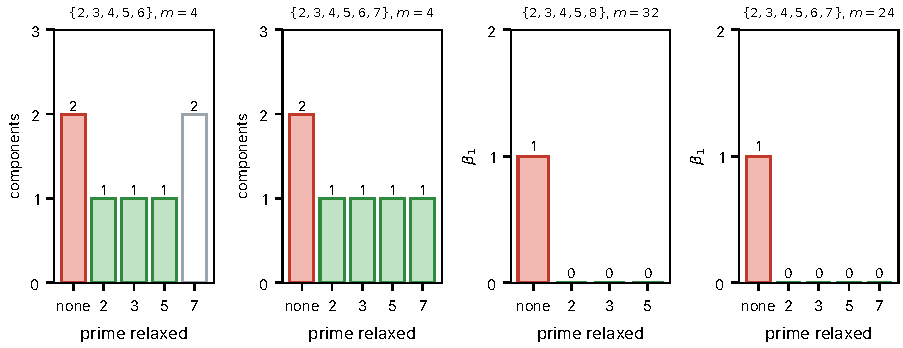
\includegraphics[width=\textwidth]{fig15_irreducible_obstructions}
\caption{\textbf{Irreducible prime-resource obstructions (exact).} For each of the four instances of \cref{prop:irred}: the number of components (panels 1--2) or the first Betti number (panels 3--4) of $K_m$ when nothing is relaxed (red bar) and when exactly one prime is relaxed (green bars). In panel~1 relaxing the passive prime $7$ (which does not constrain, by \cref{thm:passive}) is also shown and leaves $2$ components. Every active prime, relaxed alone, removes the obstruction. Theorem illustrated: \cref{prop:irred}, \cref{thm:passive}.}\label{fig:irreducible}
\end{figure}
\noindent The figure above is \cref{fig:irreducible}; its caption states the exactness of what is drawn.
\begin{proposition}[census of obstruction support; finite-exact, cited]\label{prop:supportcensus}
In the programme's census of route complexes with $k\le5$ labels (cap of $500$ resource vectors per content), disconnections occur with support $2,3,4$; loops with support $2,3$ (never $4$ for $k\le5$); voids only with support $2$; and the cut order (the least number of simultaneously relaxed primes that makes the complex contractible) is $1$ in about $17\,900$ non-trivial feature instances. This was not re-run here. Whether synergistic obstructions of cut order $\ge2$ exist is open.
\end{proposition}
\prov{CW-0386}{B-T4}{FINITE-EXACT}{FINITE}
\begin{problem}[open: repeated labels]\label{prob:repeated}
The complexes of this section and of \cref{sec:feasible} are defined for sets of distinct labels. For repeated labels the face structure of the arrangement graph needs a construction by chains of sub-multisets; none is given here, and \cref{thm:dual,thm:lower,thm:sphere} are not claimed for repeated labels. (The prefix-set form, the threshold law and \cref{thm:F2} do hold for repeated labels.)
\end{problem}
